%==============================================================================
% Sjabloon poster bachproef
%==============================================================================
% Gebaseerd op document class `a0poster' door Gerlinde Kettl en Matthias Weiser
% Aangepast voor gebruik aan HOGENT door Jens Buysse en Bert Van Vreckem

\documentclass[a0,portrait]{hogent-poster}

% Info over de opleiding
\course{Bachelorproef}
\studyprogramme{toegepaste informatica}
\academicyear{2022-2023}
\institution{Hogeschool Gent, Valentin Vaerwyckweg 1, 9000 Gent}

% Info over de bachelorproef
\title{Hoe kan het ontwikkelen van een interne applicatie het handmatig testen van een privaat netwerk vereenvoudigen?}
\author{Jasper Berton}
\email{jasper.berton@student.hogent.be}
\supervisor{Sion Verschraege}
\cosupervisor{Jens Buysse (Citymesh)}

% Indien ingevuld, wordt deze informatie toegevoegd aan het einde van de
% abstract. Zet in commentaar als je dit niet wilt.
\specialisation{Mobile \& Enterprise Development}
\keywords{Private Network, Connectivity, Android}

\begin{document}

\maketitle

\begin{abstract}
In dit project werd een interne Android-applicatie ontwikkeld met als doel het vereenvoudigen en versnellen van handmatige tests binnen private netwerken. De applicatie automatiseert hierbij de gegevensverzameling en biedt real-time analyse van kritieke opgemeten waarden zoals latentie en signaalsterkte. Tijdens tests gedurende Graspop Metal Meeting 2024 bleek de applicatie effectief in het reduceren van de verwerkingstijd en het identificeren van netwerkproblemen die anders onopgemerkt zouden blijven. Dit onderzoek toont aan dat de toepassing van interne softwareoplossingen een aanzienlijke meerwaarde biedt in het beheren en optimaliseren van private netwerken.
\end{abstract}

\begin{multicols}{2} % This is how many columns your poster will be broken into, a portrait poster is generally split into 2 columns

\section{Introductie}

Indien men een privaat netwerk handmatig wenst te testen komt dit vaak neer op een tijdrovende taak omtrent het verzamelen van ongestructureerde data.
Deze bachelorproef had als doel om een applicatie te ontwikkelen waarbij er een focus is op het automatiseren van dit test proces. Hiernaast was er ook een implementatie voor data visualisatie alvorens het verstuurd werd naar een externe database. 

\section{Probleemstelling}

Private netwerken baten bij intensieve monitoring om zo de stabiele werking er van te kunnen garanderen. Er bestaan huidige commerciële alternatieven maar deze schieten vaak te kort voor specifieke use cases.

\section{Doelstelling}

Het doel van dit onderzoek was de ontwikkeling van een proof-of-concept, dit in de vorm van een Android-applicatie met als belangrijkste pijler het vereenvoudigen van de handmatige testen door:

\begin{itemize}
    \item Geautomatiseerde gegevensverzameling: Realtime monitoren van verscheidene parameters binnen een netwerk
    \item Externe data opslag: Gebruik van een database om gegevens direct te kunnen analyseren.
    \item Gebruiksvriendelijke interface: Intuïtieve bediening voor snelle configuratie en test uitvoering.
\end{itemize}

\section{Methodologie}

De applicatie werd uitgebouwd gedurende meerdere iteraties, waarbij feedback verschillende partijen binnen Citymesh werd geïntegreerd. De applicatie werd getest op Graspop Metal Meeting 2024 om de effectiviteit binnen een real-world scenario te evalueren.

%\section{Sectie met figuur}

%De {\LaTeX} figure-omgeving bepaalt zelf waar een afbeelding komt en dat is meestal niet op de plek in de tekst waar de figure-omgeving gedefinieerd wordt. Als je wilt forceren dat afbeeldingen toch in de flow van de tekst blijven, dan kan je dat zoals hieronder:

\begin{center}
  \captionsetup{type=figure}
  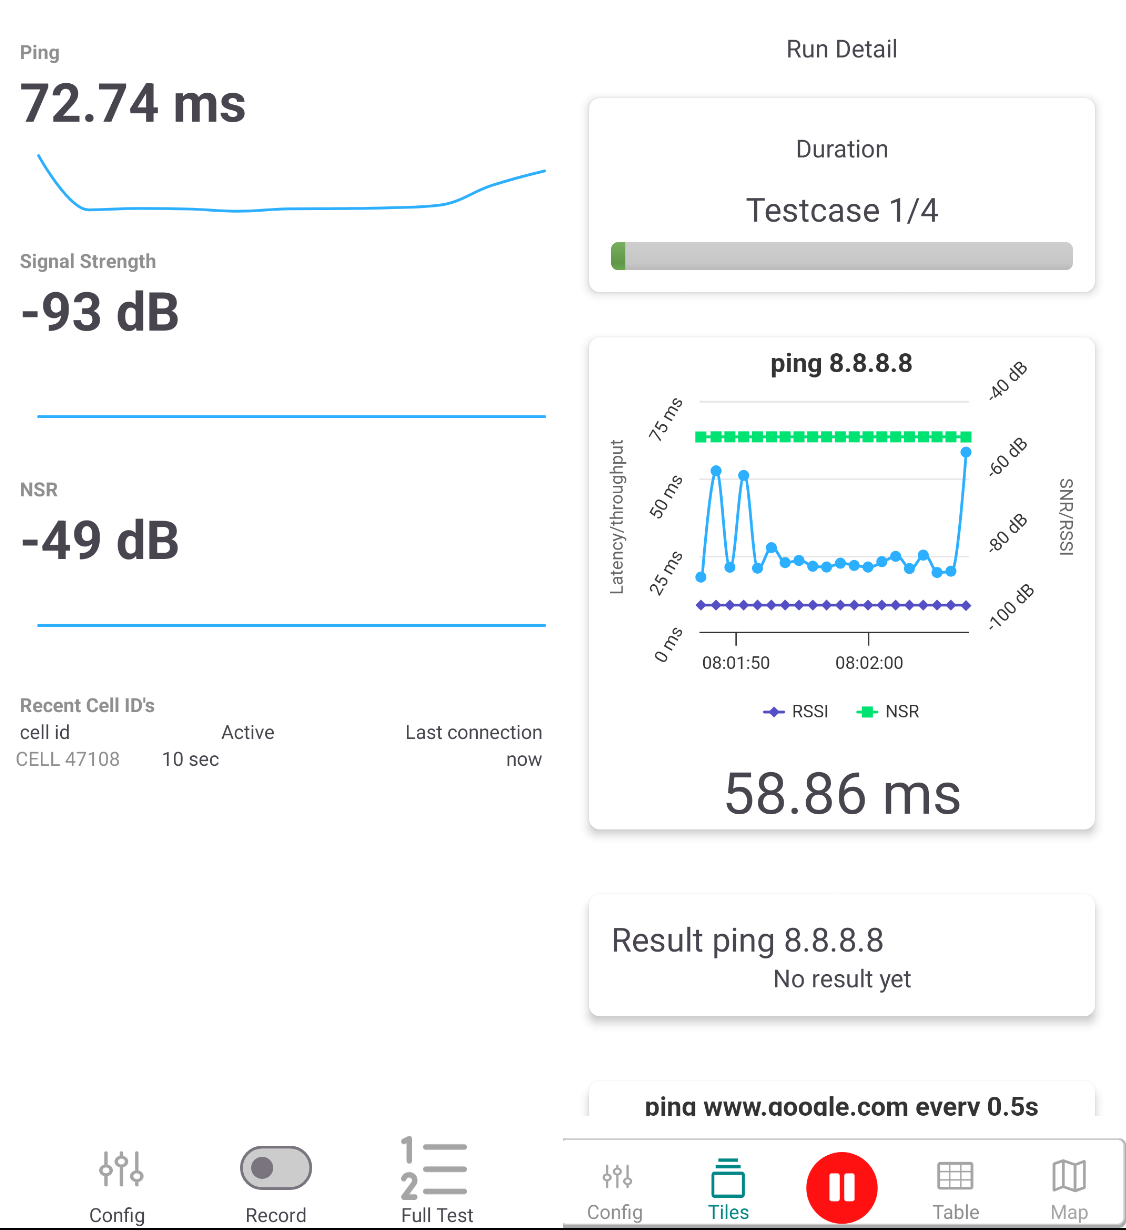
\includegraphics[width=0.7\linewidth]{continuousspecificmerge}
  \captionof{figure}{Twee schermen desbetreffende de dataverzameling binnen de proof-of-concept}
\end{center}

%Let er wel op dat dit tot problemen met bladschikking kan leiden.

\section{Resultaten}

\begin{itemize}
    \item Efficiëntieverbetering: De applicatie reduceert nodige verwerkingstijd van testdata significant.
    \item Inzichten: De ontwikkelde oplossing identificeerde netwerkproblemen die onopgemerkt bleven voor commerciële software.
    \item Gebruikservaring: De toepassing bleek gebruiksvriendelijk en flexibel inzetbaar in verscheidene netwerktests.
\end{itemize}

\section{Conclusies}

De ontwikkelde applicatie toont aan dat handmatige netwerktests aanzienlijk kunnen worden geoptimaliseerd door gebruik te maken van interne softwareoplossingen. Dit project legt de basis voor toekomstige ontwikkelingen waarbij de automatisering van netwerkbeheer verder kan worden uitgebreid.

\section{Toekomstig onderzoek}

Voor toekomstig onderzoek kan er gekeken worden naar de impact van data transfer over een netwerk gedurende de test periode. Research naar uitvoeren van testen in een passieve vorm op het apparaat is ook een pad om verder te exploreren.

\end{multicols}
\end{document}